\documentclass[a4paper,10pt]{article}

% ------------------------------------
% packages
\usepackage[a4paper,margin=1in,footnotesep=2.2\baselineskip]{geometry}
\usepackage{multicol}
\usepackage{xcolor}
\usepackage{framed}
\usepackage{emoji}
\usepackage[most]{tcolorbox}
\usepackage{fancyhdr}
\usepackage[tracking=true]{microtype}
\usepackage{ragged2e}
\usepackage{listings}
\usepackage{color}
\usepackage{pagecolor}
\usepackage{pdftexcmds}
\usepackage{geometry}
\usepackage{caption}
\captionsetup{
  font=small,
  labelfont=bf,
  tableposition=top
}
\captionsetup[figure]{name=\mono{Figure}}

% ------------------------------------
% checksum = SHA-1
\makeatletter
\ifx\pdf@filemdfivesum\undefined\def\pdf@filemdfivesum#{\mdfivesum file}\fi
\let\filesum\pdf@filemdfivesum
\makeatother

% ------------------------------------
% color definitions
\definecolor{armygreen}{rgb}{0.14, 0.71, 0.15}
\definecolor{darkgreen}{rgb}{0.08, 0.48, 0.18}
\definecolor{darkred}{rgb}{0.86, 0.153, 0.153}
\definecolor{azure}{rgb}{0.0, 0.5, 1.0}
\definecolor{bole}{rgb}{0.82, 0.57, 0.22}
\definecolor{dkgreen}{rgb}{0,0.6,0}
\definecolor{gray}{rgb}{0.5,0.5,0.5}
\definecolor{mauve}{rgb}{0.58,0,0.82}
\definecolor{light-gray}{gray}{0.95}
\definecolor{bg}{HTML}{fcfcfa}
\definecolor{bt}{HTML}{ffebe6}

% ------------------------------------
% code styling
\definecolor{shadecolor}{RGB}{180,180,180}
\newcommand{\code}[1]{\colorbox{shadecolor!30}{\mono{#1}}}
\colorlet{Gray}{gray!20!}
\tcbset{on line, arc=1pt, leftrule=0.25pt,rightrule=0.25pt,toprule=0.25pt,bottomrule=0.25pt,
	boxsep=3pt, left=0pt,right=0pt,top=0pt,bottom=0pt,
	colframe=white,colback=Gray,  
	highlight math style={enhanced}
}
\lstdefinelanguage{Solidity}{
  %keywords={bool, true, false, return, address, bytes32, bytes4, bytes1, bytes, uint256, uint8, uint, string, if, while, else, case, break},
  keywords={},
  keywordstyle=\color{blue}\bfseries,
  %ndkeywords={function,struct, mapping, export, throw, implements, import, this},
  ndkeywords={},
  ndkeywordstyle=\color{darkgreen}\bfseries,
  identifierstyle=\color{black},
  sensitive=false,
  comment=[l]{//},
  morecomment=[s]{/*}{*/},
  commentstyle=\color{green}\mono,
  stringstyle=\color{orange}\mono,
  morestring=[b]',
  morestring=[b]",
  mathescape=true,
  literate={=>}{$\rightarrow{}$}{1}
}
\lstset{
  backgroundcolor=\color{light-gray},
  language=Solidity,
  aboveskip=3mm,
  belowskip=3mm,
  showstringspaces=false,
  columns=flexible,
  basicstyle={\footnotesize\mono},
  numbers=none,
  numberstyle=\tiny\color{gray},
  keywordstyle=\color{blue},
  commentstyle=\color{dkgreen},
  stringstyle=\color{mauve},
  breaklines=true,
  breakatwhitespace=true,
  tabsize=3
}

% ------------------------------------
% fonts
\newfontfamily\pro[Path=./]{SFMono.ttf}
\newfontfamily\pbold[Path=./]{SFMonoBold.ttf}
\newfontfamily\mono[Path=./]{SFMono.ttf}
\newfontfamily\mbold[Path=./]{SFMonoBold.ttf}

% ------------------------------------
% heading font-size
\usepackage{sectsty}
\usepackage{fontspec}
\sectionfont{\fontsize{12}{15}\selectfont}
\usepackage[utf8]{inputenc}

% ------------------------------------
% footnote positioning
\usepackage[hang,flushmargin,bottom]{footmisc} 

% ------------------------------------
% bibliography
\usepackage[colorlinks=true,
            linkcolor=blue,
            urlcolor=blue,
            citecolor=blue,
            pdfauthor={sshmatrix},
            pdftitle={Helix2 Protocol},
            pdfsubject={Link Service and Protocol},
            pdfkeywords={ethereum, account, abstraction, link, name, decentralised, distributed},
            pdfproducer={sshmatrix},
            pdfcreator={sshmatrix}]{hyperref}
            
% ------------------------------------
% blank footnote
\newcommand\blfootnote[1]{%
	\begingroup
	\renewcommand\thefootnote{}\footnote{#1}%
	\addtocounter{footnote}{-1}%
	\endgroup
}

% ------------------------------------
% header
\pagestyle{fancy}
\fancyhf{}
\lfoot{\footnotesize \mono{\#}\tcbox{\mono{\filesum{\jobname}}}}
\begin{document}
\setcounter{footnote}{0}
\newpage
\topskip15pt

\fancyhead[L]{\footnotesize \mono{author}:\tcbox{\mono{sshmatrix}}}
\fancyhead[R]{{\footnotesize \mono{\href{https://github.com/sshmatrix/research}{github.com/sshmatrix/research/zkReview}}}}
\fancyhead[C]{{\footnotesize \emoji{dna}}}
\fancyfoot[C]{{\footnotesize \mono{\thepage/-}}}
\fancyfoot[R]{{\footnotesize \mono{\today} \emoji{dna}}}

\begin{center}
	\textbf{\Large\pbold{\textls[-40]{Intuitive Interpretation of Non-Interactive Zero-Knowledge Cryptography}}}\\
	\vspace{0.075in}
	\textls[-50]{\mono{A jargon-free approach to understanding zk-SNARKs and zk-STARKs}}\linebreak\linebreak
	\vspace{-0.175in}
	\textls[0]{\mono{Avneet Singh}}\linebreak\linebreak
	\textls[0]{\mono{Interplanetary Company UG}}\linebreak
	\textls[0]{\mono{\href{mailto:sshmatrix@proton.me}{sshmatrix@proton.me}}}\linebreak
\end{center}
\begin{center}
	\textbf{\Large\pbold{ABSTRACT}}\linebreak\linebreak
	\textls[-50]{\mono{zk-SNARKs and zk-STARKs are relatively new concepts in cryptography, yet they are being touted as the next forefront in modern and future crypto tech. In blockchain space specifically, there is great interest in these subfields in the context of zk-Rollups to Layer 1 blockchains such as Ethereum, or as standalone decentralised ledgers with high rates of transactions per second (TPS), e.g. Aztec Network (zk-STARK), zkSync, Loopring, ZCash (zk-SNARKs) etc. Despite their great importance in cryptography, it is unfortunately difficult to understand zk-SNARKs and zk-STARKs due to limited literature and conceivably difficult mathematics conveyed through intensive jargon. This paper is an attempt to introduce zero-knowledge (zk) cryptography in an intuitive manner to garden-variety mathematicians, physicists, curious blockchain developers and perhaps even cryptographers.}}
\end{center}
\vspace{0.2in}
\begin{flushleft}
	\textbf{\Large\pbold{INTRODUCTION}}\linebreak\linebreak
	\textls[-50]{\mono{Zero-knowledge cryptography is presumably the next natural stage in cryptography's evolution toward post-quantum era. zk-SNARKs and zk-STARKs are specific implementations of zero-knowledge cryptography that are widely considered the most promising path toward post-quantum security. In order to deeply understand zero-knowledge cryptography, one must at least understand the current generation cryptographic systems such as RSA (Rivest–Shamir–Adleman) and Elliptic Curve Cryptography (ECC); this is admittingly a challenging task since the mathematics of such protocols is rather tedious and it only gets exponentially worse as one ventures in zero-knowledge protocols. Despite these challenges, it is nonetheless easier to understand at least the philosophy and intuition behind zero-knowledge protocols using the famous Alibaba Cave example [1] without requiring any prerequisite knowledge of RSA or ECC. We leave this as an exercise for the reader. In this paper, we will attempt to delve into the practical implementation of zero-knowledge protocols while retaining an intuitive understanding of the underlying mathematical processes.\linebreak\linebreak
	}}
	\colorbox{Gray}{\hspace{1mm}\parbox{0.99\textwidth}{\vspace{1mm}\textls[-50]{\mono{Through the course of this paper, we will leave additional comments in a grey box targeted at physicists, mathematicians and developers. These comments are anecdotes, comparisons or similariries noted across different fields that may help readers develop an intuitive understanding.\vspace{1mm}}}}}
\end{flushleft}
\begin{flushleft}
	\textls[-50]{\mono{Cryptographic protocols at their core are motivated by the need to prove access to some information without necessarily revealing a part or the entirety of said information. In mathematical terms, there are several ways of achieving this functionality from an intelligently designed system.\linebreak
	}}
\end{flushleft}
\begin{flushleft}
	\textbf{\large\pbold{PRIME NUMBERS}}\linebreak\linebreak
	\textls[-50]{\mono{Cryptographers realised back in the day that prime numbers were one such system that could provide the desired functionality. For instance, consider two sufficiently large prime numbers {\pbold{a}} = 53781811 and {\pbold{b}} = 23252729, and their even larger product {\pbold{a}}$\,\times\,${\pbold{b}} = 1250573876312219. The product 1250573876312219 is a relatively difficult number to prime factorise back to {\pbold{a}} and {\pbold{b}} if both {\pbold{a}} and {\pbold{b}} are unknown. However, if either one of the two prime factors ({\pbold{a}} or {\pbold{b}}) are known, then it is straightforward to calculate the other unknown prime factor by simple division. To intuitively understand this system further, let's break it down into its principle components: we took a set of very large prime numbers of which {\pbold{a}} and {\pbold{b}} are members and defined an operation of multiplication\textsuperscript{\textcolor{blue}{1}}\blfootnote{\textls[-50]{\mono{\textsuperscript{1}in addition to implicitly defining the operation of addition '+' and its inverse subtraction '-'}}} on the members of the set; such a finite field is called a Galois field. Additionally, we note that the product operation $\times$ is difficult to invert unless one of the two numbers is known; this kind of a system is usually called a trapdoor.\linebreak\linebreak 
	}}
	\colorbox{Gray}{\hspace{1mm}\parbox{1.0\textwidth}{\vspace{1mm}\textls[-50]{\mono{In abstract mathematics, such a system is called a Group and the study of groups is called Group theory; a group is defined by a set of elements (called a Field, e.g. large prime numbers) along with the set of permitted operations between those elements (e.g. multiplication). The configuration of any trapdoor system is such that the permitted operations defined on the elements of the group are difficult to invert.\vspace{1mm}}}}}\linebreak\linebreak\linebreak
	\textls[-50]{\mono{This trapdoor feature of our chosen system is essentially the backbone of all present day cryptography.\linebreak\linebreak
	}}
	\textbf{\Large\pbold{RSA CRYPTOGRAPHY}}\linebreak\linebreak
	\textls[-50]{\mono{RSA protocol is one of the simplest implementations of the trapdoor feature which results in a keypair system - a public key and a private/secret key - typically utilised in conjunction for encrypting and decrypting information. The premise of the RSA protocol essentially lies in setting, i) public key as the qualitative equivalent of the product {\pbold{a}}$\,\times\,${\pbold{b}}, and ii) private key as the qualitative equivalent of either {\pbold{a}} or {\pbold{b}}, where {\pbold{a}} and {\pbold{b}} are restricted to a finite field of prime numbers (denoted by F\textsubscript{\pbold{p}}). The security of such a system is encoded in the difficulty of prime factorising the product. It is unimportant to know the precise details of the protocol implementation in context of this paper. In nutshell, the RSA algorithm requires solving for the coefficients (x,\,y) of Bezout's Identity (x\,{\pbold{a}} + y\,{\pbold{b}} = 1) using extended Euclidean algorithm [2] and employing modular arithmetic to wrap integer numbers when they fall outside a separately defined finite prime field F\textsubscript{\pbold{p'}}.\linebreak\linebreak
	}}
	\colorbox{Gray}{\hspace{1mm}\parbox{1.0\textwidth}{\vspace{1mm}\textls[-50]{\mono{Modular arithmetic is quite simply equivalent to adding the modulo '\%' operation over some prime number {\pbold{p}} to all group operations $\bullet$ (i.e. $\bullet$ = $+$, $-$, $\times$ or $/$), such that {\pbold{a}} $\bullet$ {\pbold{b}} $\rightarrow$ {\pbold{a}} $\bullet$ {\pbold{b}} \% {\pbold{p}}. Modular airthmetic is regular arithmetic 'wrapped' by the modulo operator such that results of all group operations lie within 0 and {\pbold{p}}.\vspace{1mm}}}}}\linebreak\linebreak\linebreak
	\textbf{\large\pbold{ROBUSTNESS OF RSA}}\linebreak\linebreak
	\textls[-50]{\mono{While RSA is sufficiently safe to use today, it's safety will decrease over time as computational capacity of human civilisation increases. This is because the fastest and - arguably - maximally efficient algorithms capable of inverting the {\pbold{a}}$\,\times\,${\pbold{b}} product are iterative by construction and rely on optimised brute-forcing; Quadratic Sieve [3] and General Number Field Sieve [4] are two such well-known methods. With the advent of quantum computers, RSA algorithm's security will be definitively compromised; this is the so called SNDL problem (Save-Now-Decrypt-Later) facing the cryptography community today [5]. The core issue at hand here is that finite prime fields and the generic operation of multiplication on them - irrespective of the largeness of its elements - does not possess sufficient difficulty if the exploitor has relatively large computational resources at hand. In order to design better cryptosystems that are secure against brute-forcing, one must come with a new group with a better choice of finite field and a preferably a harder group operation which is resistant to such an attack.\linebreak\linebreak 
	}}
	\textbf{\large\pbold{DIFFIE-HELLMAN KEY EXCHANGE}}\linebreak\linebreak
	\textls[-50]{\mono{In very few lines, let us discuss the Diffie-Hellman Key Sharing Algorithm. Diffie-Hellman is another cryptosystem which in some sense is the intermediate step between RSA and ECC since it introduces finite fields over groups other than itself. In simple terms, this means that the group operation of product $\times$ remains the same but the group elements are now that of a finite cyclic group [6]. The non-invertible term securing the protocol in this case is of the form\textsuperscript{\textcolor{blue}{2}}\blfootnote{\textls[-50]{\mono{\textsuperscript{2}{\pbold{G}} is called the group generator (integer), {\pbold{K}} is private key (integer) and {\pbold{p}} is a prime number}}} {\pbold{G}}\textsuperscript{\pbold{K}} \% {\pbold{p}}, instead of a simple product between two large prime numbers. Breaking the Diffie-Hellman method is thereby different from RSA since it involves inverting {\pbold{G}}\textsuperscript{\pbold{K}} \% {\pbold{p}} instead of {\pbold{a}}$\,\times\,${\pbold{b}}; this is known as the discrete logarithm problem.\linebreak\linebreak
	}}
	\colorbox{Gray}{\hspace{1mm}\parbox{1.0\textwidth}{\vspace{1mm}\textls[-50]{\mono{Note that the term {\pbold{G}}\textsuperscript{K} is better not interpreted as a literal exponent although a lot of literature uses this terminology. {\pbold{G}}\textsuperscript{\pbold{K}} is a representation for a group operation that 'operates on or with itself' {\pbold{K}} number of times. In context of cyclic groups, {\pbold{G}} is the generator element of the group (of order N), i.e. the element from which all other elements can be derived by iteratively performing the {\pbold{G}}\textsuperscript{\pbold{K}} operation for {\pbold{K}} = 1, 2, 3 ... N.\vspace{1mm}}}}}\linebreak\linebreak\linebreak
	\textbf{\Large\pbold{ELLIPTIC CURVE CRYPTOGRAPHY}}\linebreak\linebreak
	\textls[-50]{\mono{The fundamental issue that leads to the breakdown of RSA algorithm is that the prime number field and the operation of multiplication is not complex enough in the face of large computational power. The effort to improve on this problem led to the advent of Elliptic Curve Cryptography (ECC). ECC functions by fixing the core illnesses in RSA, i.e. it proposes - similar to Diffie-Hellman - that instead of operating on the prime number field itself, we operate on another field on which we define a newer set of operations that are much harder to invert. The premise of ECC thus lies in the introduction of finite prime fields over elliptic curves, a step up from finite cyclic groups used in Diffie-Hellman [7]. In context of cryptography, an Elliptic curve is simply the following relation between two finite prime fields ({\pbold{x}}, {\pbold{y}}),}}
	\begin{center}
		{\mono{{\pbold{y}}\textsuperscript{2} = {\pbold{x}}\textsuperscript{3} + p\,{\pbold{x}} + q, \\
		\vspace{2mm}
		given 4\,p\textsuperscript{3} + 27\,q\textsuperscript{2} $\neq$ 0
		}}
	\end{center}
	\begin{flushright}
		{\vspace{-8mm}\mono{(1)}}
	\end{flushright}
	\textls[-50]{\mono{Gigabrains realised few decades ago that the elliptic curves have some very cool properties in context of invertibile binary operations. To begin with,\linebreak\linebreak
	1. The elliptic curve is symmetric across the x-axis; this is a desirable property since it ensures the existence of both {\pbold{y}} and -{\pbold{y}} in our group. More importantly,\linebreak
	2. For any two points {\pbold{a}} and {\pbold{b}} on the elliptic curve, a line through them intersects the elliptic curve again at most - but not necessarily - 1 more point, denoted by {\pbold{c}}; the blue line in figure \ref{fig:ecc0} is one such example.\linebreak\linebreak
	}}
\end{flushleft}
\begin{multicols}{2}
	\noindent
	\begin{minipage}{\linewidth}
		\centering
		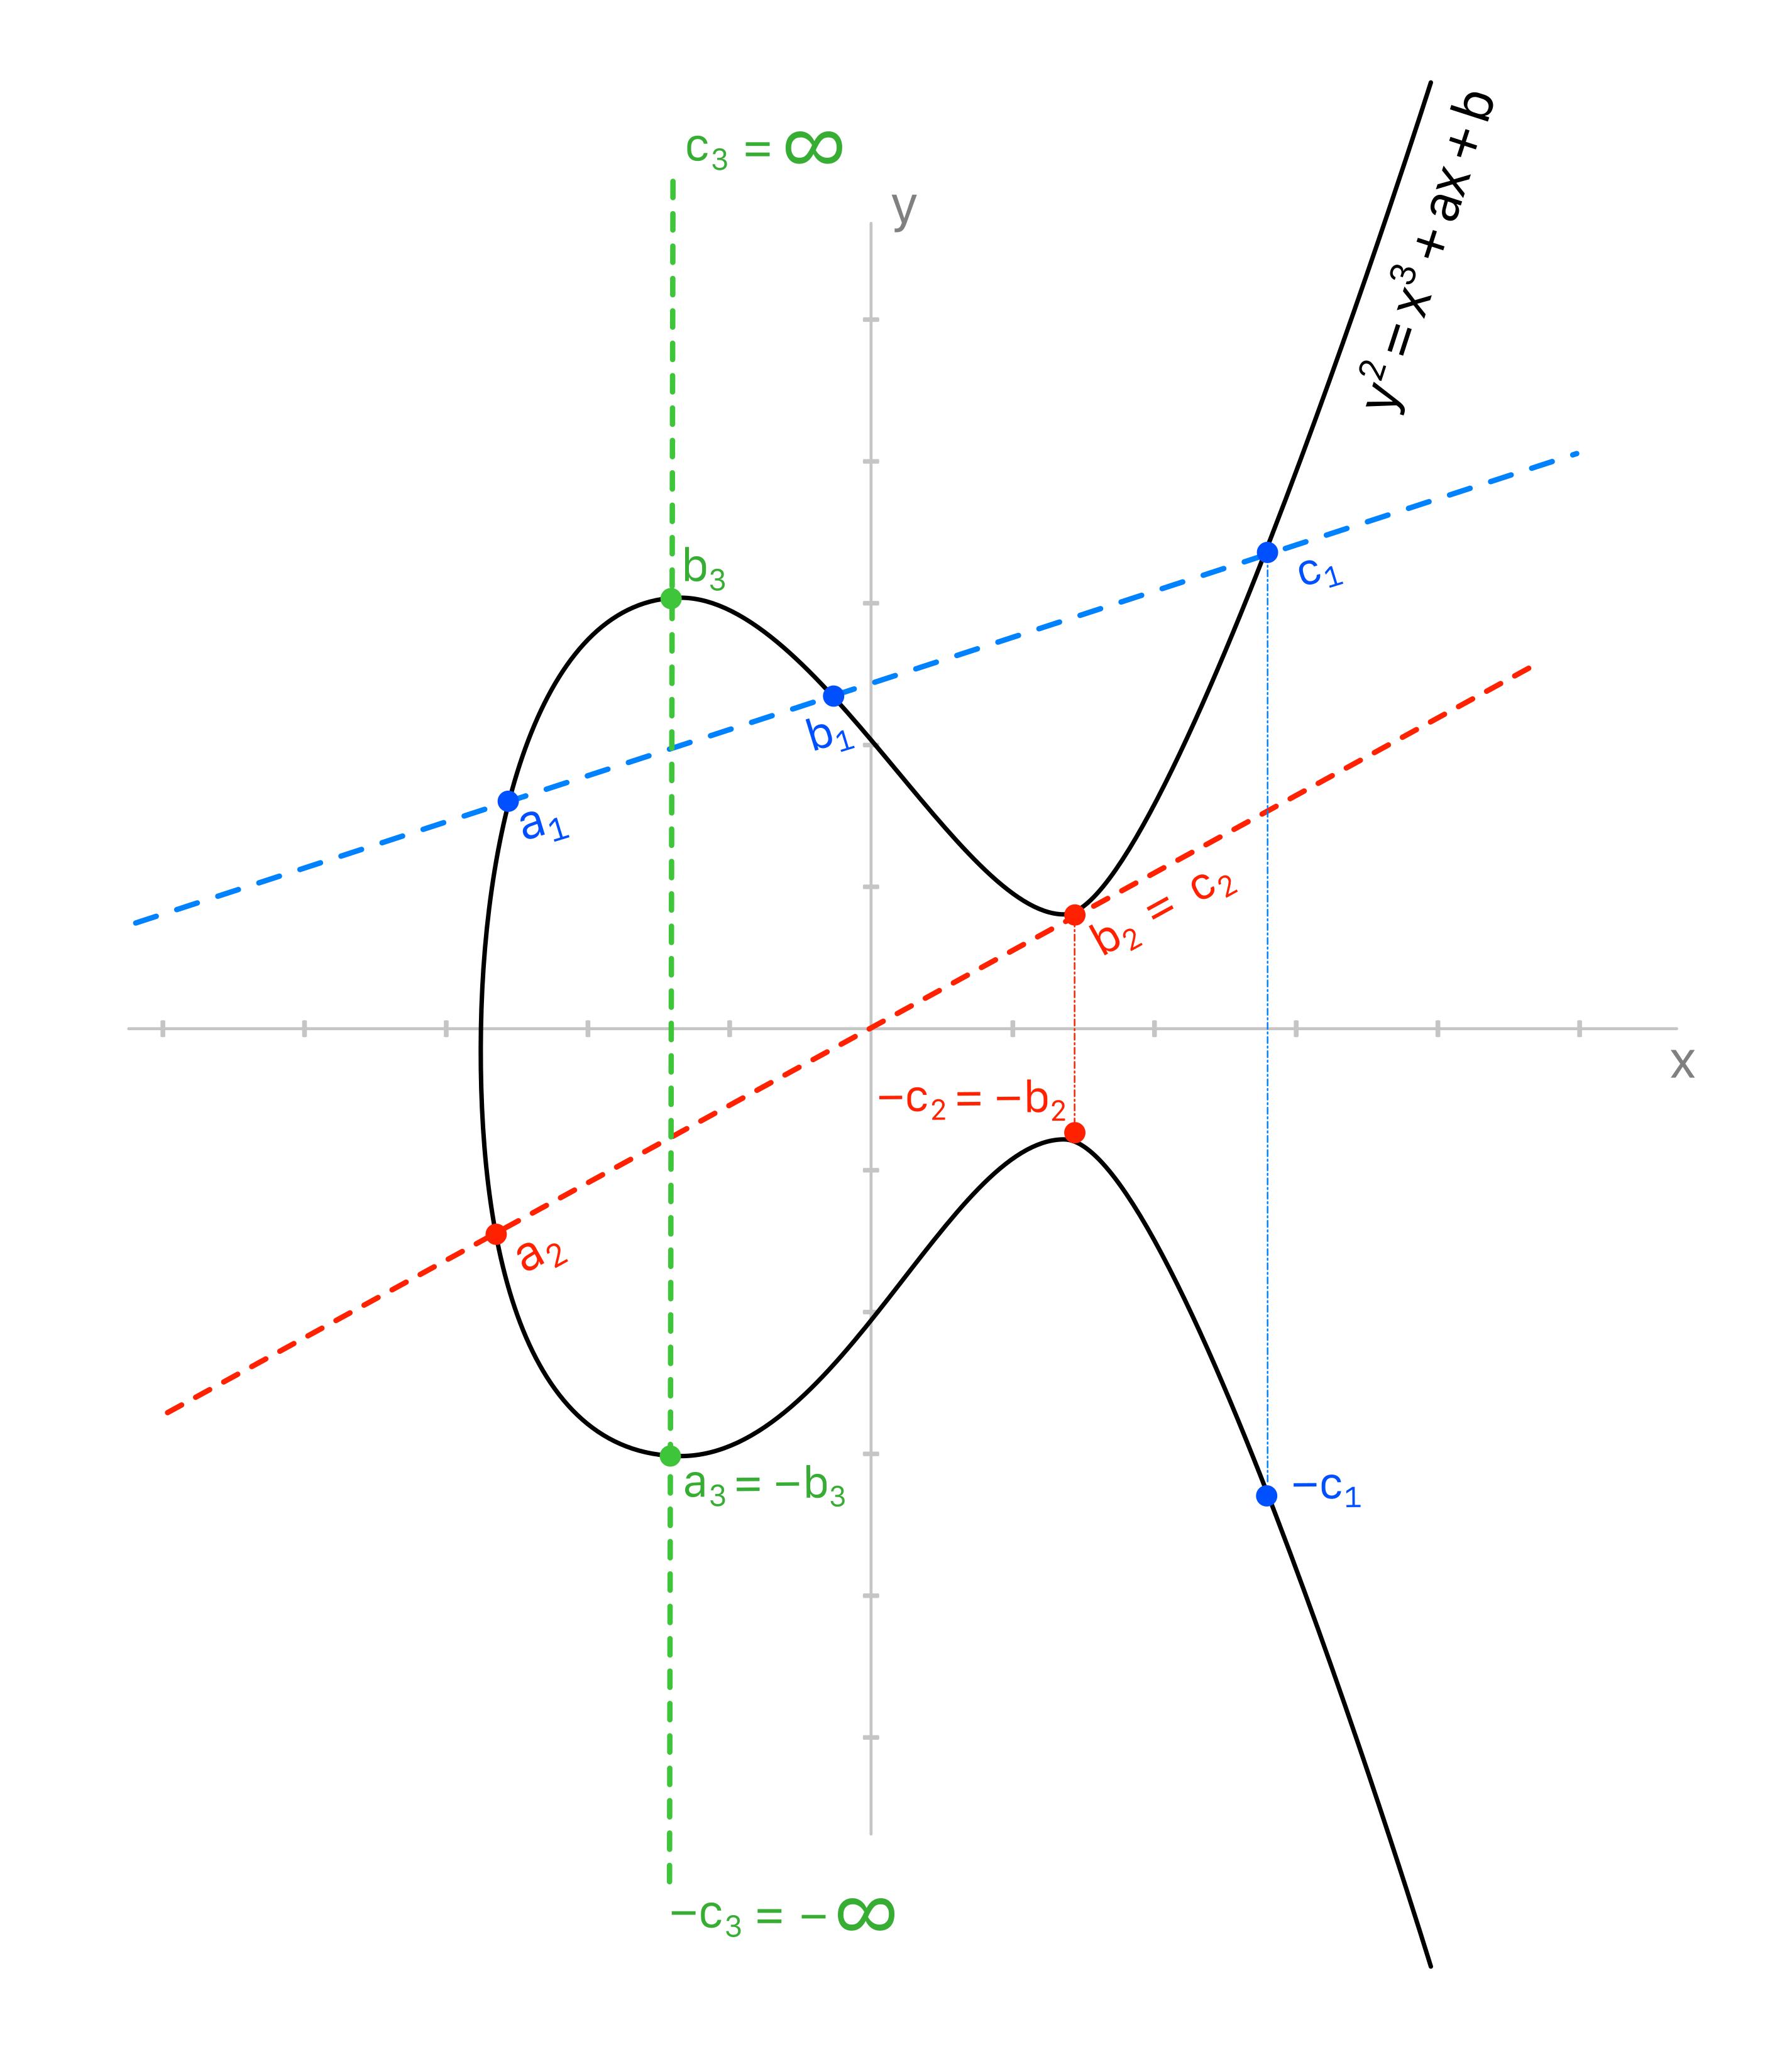
\includegraphics[width=80mm]{ellipticCurve.png}
		\captionof{figure}{\mono{Elliptic curve over a continuous infinite field, aka a Lie group. We ignore the finite field contraint in this figure for simplicity.}}
		\label{fig:ecc0}
	\end{minipage}
	\noindent
	\begin{minipage}{\linewidth}
		\centering
		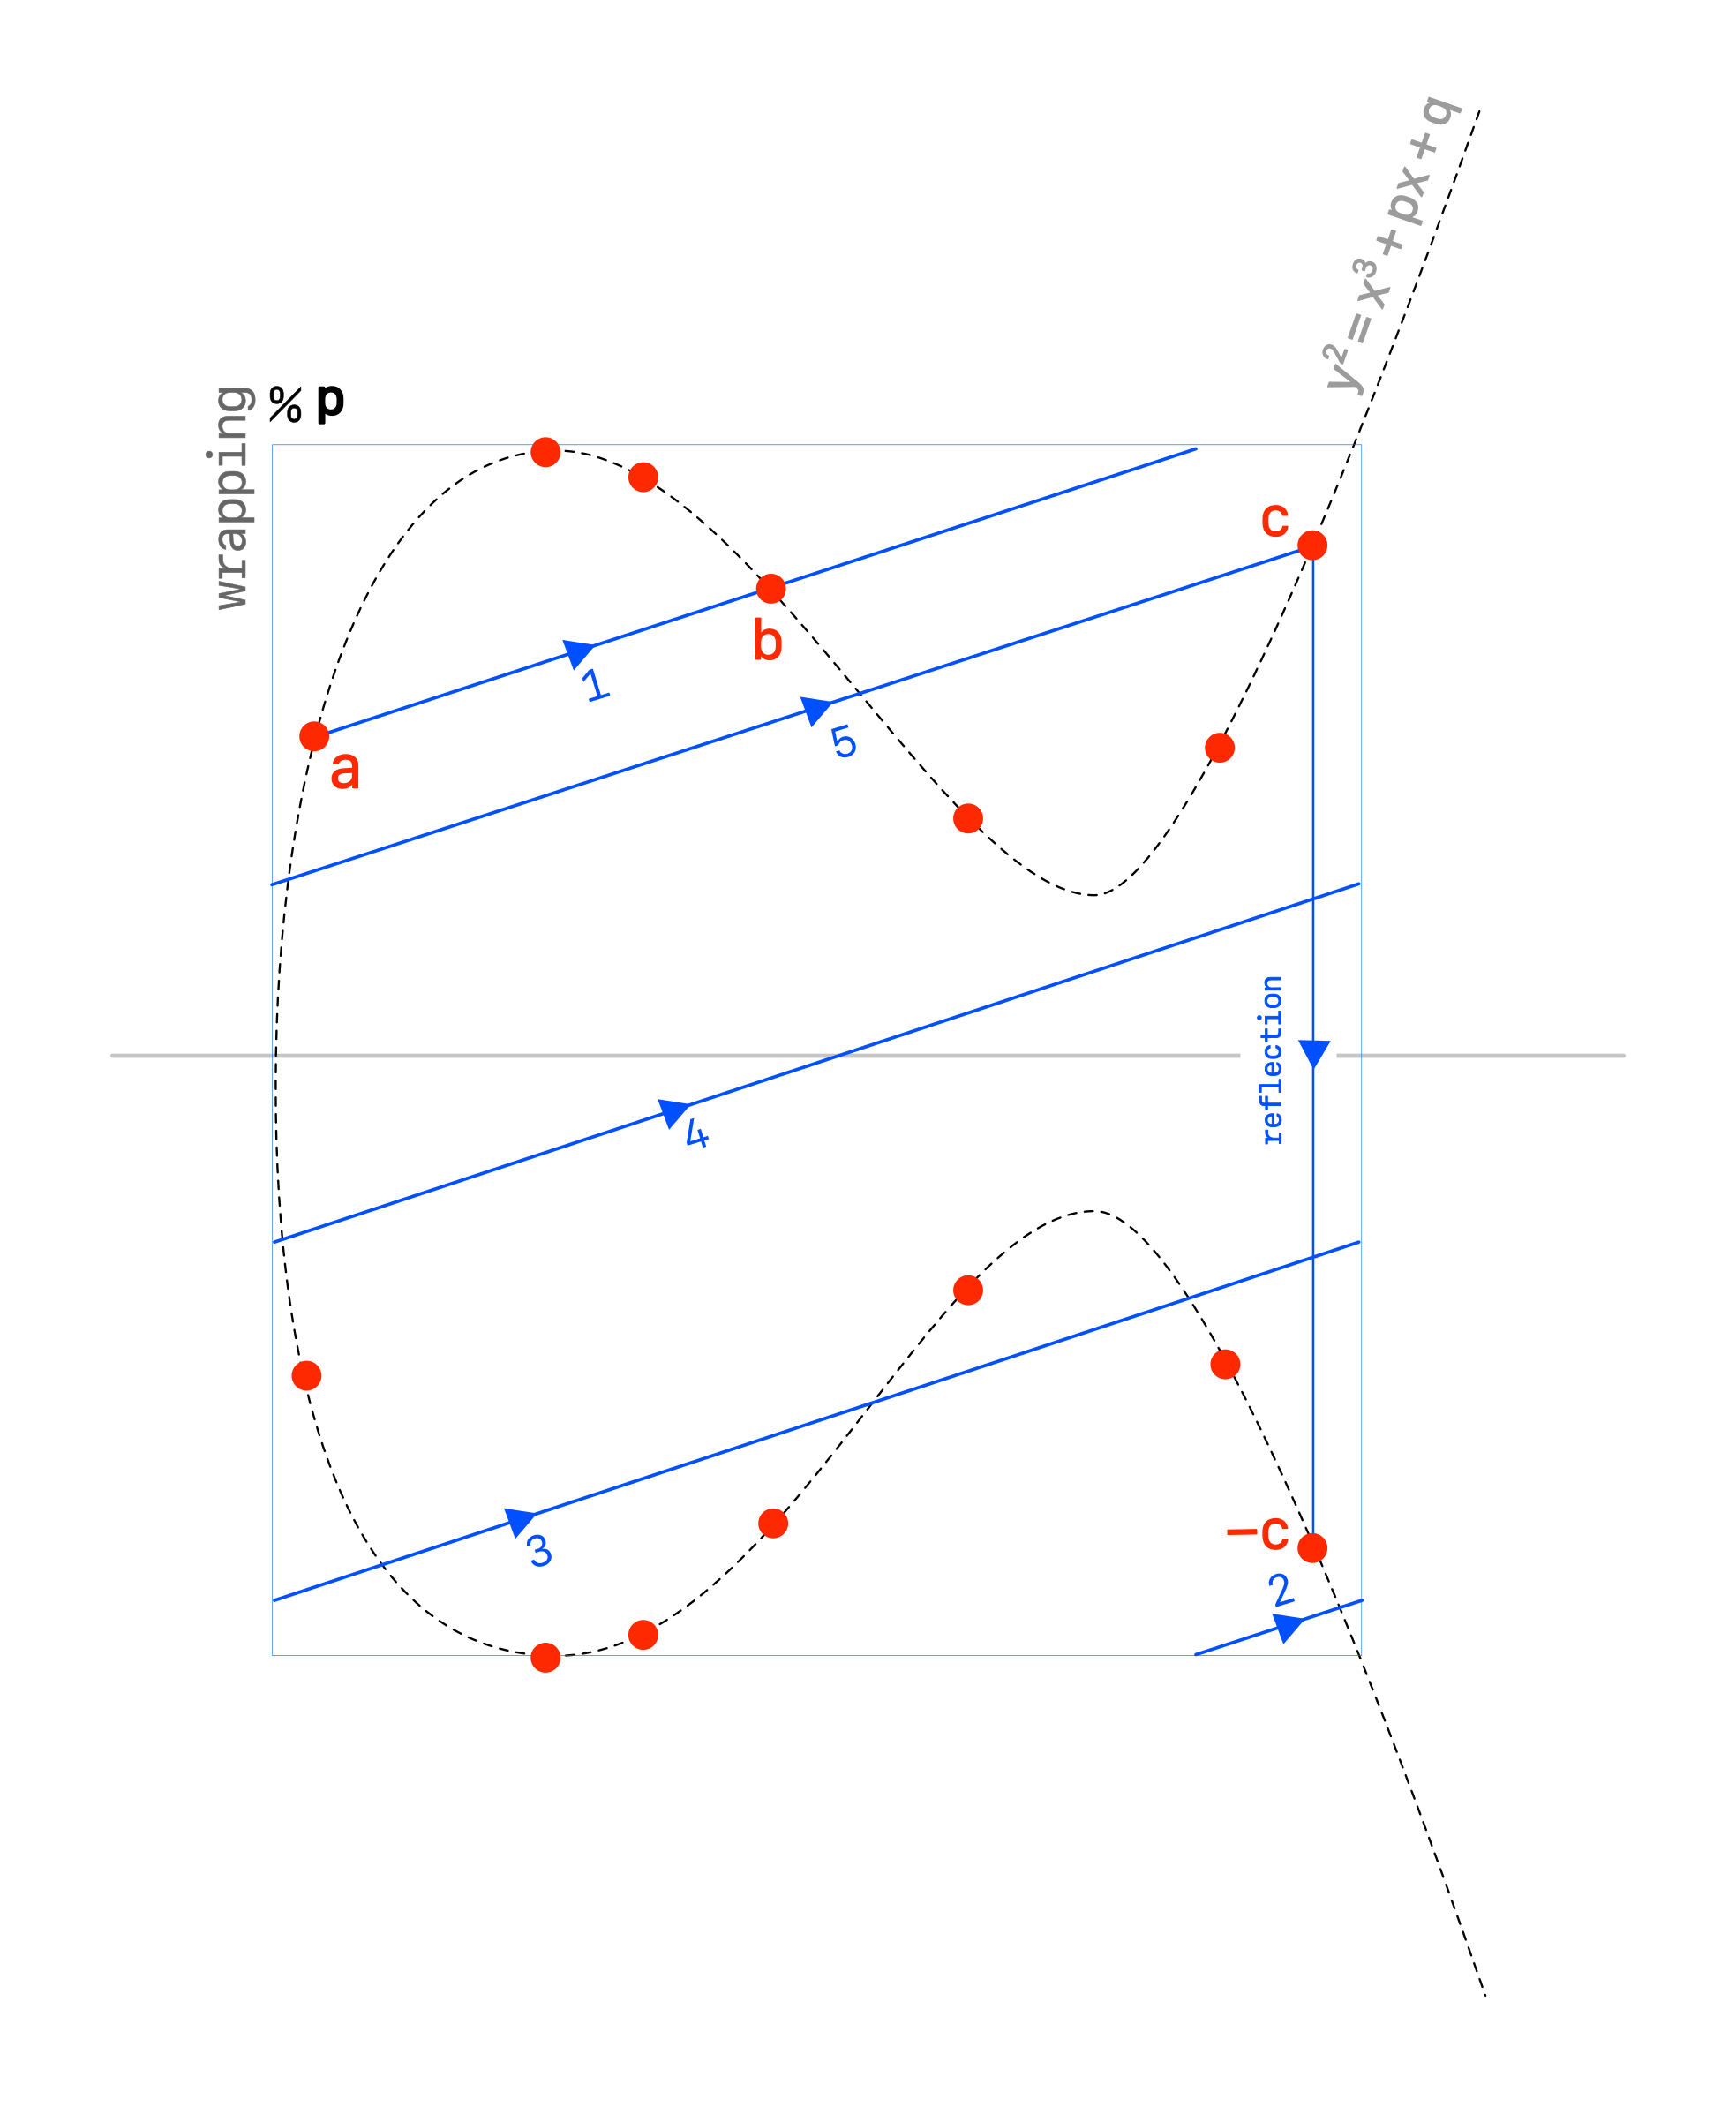
\includegraphics[width=80mm]{ECC.png}
		\captionof{figure}{\mono{Elliptic curve over a finite prime field modulo {\pbold{p}}; the effect of the modulo operator \% is to "wrap" the out-of-range values to within range. In the above example, it takes 5 'wrappings' and 1 final reflection to calculate -{\pbold{c}}.}}
		\label{fig:ecc1}
	\end{minipage}
\end{multicols}
\begin{flushleft}
	\textls[-50]{\mono{Typically, {\pbold{x}} is taken as the independent finite prime field and {\pbold{y}} is the so-called 'elliptic curve (evaluation) over finite field'; {\pbold{y}} are the elements of our desired new group. Ignoring the finite field constraint for a moment, the elliptic curve is shown in figure \ref{fig:ecc0} when {\pbold{x}} is a continuous real variable. Our task now is to come up a hard-to-invert group operation on the continuous elements {\pbold{y}} of our new group; we will reinstate the finite prime field constraint afterwards.
	}}
	\textls[-50]{\mono{Note that it is possible for the line to not intersect the curve for the third time at all, and these singularities are in fact necessary for our group to function. Consider, the green line in figure \ref{fig:ecc0}; note that all vertical lines intersect the curve at exactly two points. It is also possible for a tangent to the curve to intersect the curve at exactly two points; see one such example (the red line) in figure \ref{fig:ecc0}. The aforementioned gigabrains soon realised that one can use this intersectional property of a line with the elliptic curve (aka properties 1. and 2.) as the new group operation $\oplus$ such that
	}}
	\begin{center}
		\mono{{\pbold{a}} $\oplus$ {\pbold{b}} = \,-{\pbold{c}}}
	\end{center}
	\begin{flushright}
		{\vspace{-8mm}\mono{(2)}}
	\end{flushright}
	\textls[-50]{\mono{This is the same as saying that $\oplus$ operation between {\pbold{a}} and {\pbold{b}} is equivalent to taking reflection (-) of the third intersection point {\pbold{c}} across x-axis. Most literature phrases this $\oplus$ operation as the new "addition" operation on the group elements of {\pbold{y}}. However, we noted before that the third intersection {\pbold{c}} doesn't exist for all pairs {\pbold{a}} and {\pbold{b}}; in jargon-speak, we say that 'the group is not closed under the $\oplus$ operation'.
	}}
	\textls[-50]{\mono{We can solve this closeness problem by explicitely including the infinity element $\infty$ to the group. Once we have access to $\infty$, all intersections similar to the green line are assumed to intersect the curve again at {\pbold{c}} = $\infty$, such that
	}}
	\begin{center}
		\mono{{\pbold{a}} $\oplus$ $\infty$ = {\pbold{a}}}
	\end{center}
	\begin{flushright}
		{\vspace{-8mm}\mono{(3)}}
	\end{flushright}
\end{flushleft}
\begin{flushleft}
	\textls[-50]{\mono{Note that $\infty$ acts like the identity element \^I of our new group since it satisfies {\pbold{a}} $\oplus$ \^I = {\pbold{a}}. Lastly, the third case of the red line is not difficult since it is simply a special case of the blue line when {\pbold{b}} = {\pbold{c}}; another important tangent case arises when {\pbold{a}} = {\pbold{b}}, such that {\pbold{a}} $\oplus$ {\pbold{a}} = {\pbold{c}}. Now we have all the ingredients required to construct a robust inverse problem on our new group {\pbold{y}} with the permitted operation $\oplus$. We reinstate the requirement of evaluating the elliptic curve on a finite prime field by explicitely defining a finite field range and wrapping the out-of-range evaluations over the elliptic curve with the modulo operator \% {\pbold{p}}. The final form of the $\oplus$ operation is shown in figure \ref{fig:ecc1}. In a real world ECC implementation, this process is carried out a large number of times (assuming {\pbold{a}} = {\pbold{b}}, i.e. take tanget at point {\pbold{a}}) making the forward process increasingly complex but computable and the resulting inverse problem increasingly difficult to solve.\linebreak\linebreak
	}}
	\colorbox{Gray}{\hspace{1mm}\parbox{1.0\textwidth}{\vspace{1mm}\textls[-50]{\mono{In literature, you will often find the operation $\oplus$ equated to the generic addition $+$. This is not surprising since equations (2) and (3) resemble a + b = c and a + 0 = a for generic real numbers; 0 is the identity element of the $+$ operation. Having said that, in practice $\oplus$ operation is nothing like the addition operation $+$; the apparent similarity lies in their algebraic representations only. For instance, equations (2) and (3) also resemble a $\times$ b = c and a $\times$ 1 = a for generic real numbers. In this case, 1 is the identity element of the $\times$ operation. This difference in notation is a major source of confusion for the readers. In the end, $\oplus$ should not be compared to either $+$ or $\times$.\vspace{1mm}}}}}\linebreak\linebreak\linebreak
	\textls[-50]{\mono{The 'large number of repetitions' is assigned as the secret private key K\textsubscript{sec} and the public key K\textsubscript{pub} is equivalent to calculating {\pbold{a}} $\oplus$ {\pbold{a}} at a public value {\pbold{a}} = {\pbold{a}}\textsubscript{o} repeated N number of times\textsuperscript{\textcolor{blue}{4}}\blfootnote{\textls[-50]{\mono{\textsuperscript{4}{\pbold{a}} = {\pbold{b}} assertion is made purely for simplicity since having {\pbold{a}} $\neq$ {\pbold{b}} doesn't provide extra security and in fact makes forward computation unnecessarily involved.}}}, i.e. K\textsubscript{pub} = (...(({\pbold{a}}\textsubscript{o} $\oplus$ {\pbold{a}}\textsubscript{o})\textsubscript{1} $\oplus$ {\pbold{a}}\textsubscript{o})\textsubscript{2} $\oplus$ {\pbold{a}}\textsubscript{o})\textsubscript{3} ...)\textsubscript{N}. The exact inverse problem - called the elliptic curve discrete logarithm problem - is equivalent to finding the number of repetitions it took to arrive at K\textsubscript{pub} from a publicly known value {\pbold{a}}\textsubscript{o}. Is this inverse problem hard? It appears that given knowledge of K\textsubscript{pub} and {\pbold{a}}\textsubscript{o}, one can easily revert the process described in figure \ref{fig:ecc1} and derive key K\textsubscript{sec}. This is indeed true and the inverse problem only becomes hard when the coefficients in equation (1) are restricted to the prime field F\textsubscript{\pbold{p}}; more on this in the next subsection. Some of the popular elliptic curves today are specifically \code{ed25519} and \code{secp256k1}, with the later being more recent and more robust than the former.\linebreak\linebreak
	}}
	\colorbox{Gray}{\hspace{1mm}\parbox{1.0\textwidth}{\vspace{1mm}\textls[-50]{\mono{The name of the inverse problem for ECC, i.e. elliptic curve discrete logarithm problem, is highly misleading and results from purely notational reasons. The term 'logarithm' originates from interpreting the result of N times repetition of {\pbold{a}} $\oplus$ {\pbold{a}} operation as K\textsubscript{pub} = {\pbold{a}}\textsuperscript{N}.\vspace{1mm}}}}}\linebreak\linebreak\linebreak
	 \textls[-50]{\mono{It now appears that we have achieved what we set out to do: we have found a new group who elements are now values {\pbold{y}} evaluated over the finite prime field F\textsubscript{\pbold{p}} and the new group operation (...(({\pbold{a}}\textsubscript{o} $\oplus$ {\pbold{a}}\textsubscript{o})\textsubscript{1} $\oplus$ {\pbold{a}}\textsubscript{o})\textsubscript{2} $\oplus$ {\pbold{a}}\textsubscript{o})\textsubscript{3} ...)\textsubscript{N} ($\equiv$ {\pbold{a}}\textsubscript{o}\textsuperscript{N}) is very difficult to invert. We note that the result of $\oplus$ operation on the group elements results in a value which is also a member of the group\textsuperscript{\textcolor{blue}{5}}\blfootnote{\textls[-50]{\mono{\textsuperscript{5}group is referred to as 'closed under the operation $\oplus$'}}}; this was not the case in RSA scheme where the result {\pbold{a}}$\,\times\,${\pbold{b}} is never a member of the group.\linebreak\linebreak
	}}
	\textbf{\large\pbold{ROBUSTNESS OF ECC}}\linebreak\linebreak
	\textls[-50]{\mono{The natural question to ask here is: how robust is ECC when compared to RSA and Diffie-Hellman? We remember from previous section that the inverse problem in ECC only becomes hard when the coefficients p and q in equation (1) are also restricted to a large prime field F\textsubscript{\pbold{p'}}. To understand why this happens, simply note that for large prime values of {\pbold{p}}, {\pbold{q}} and {\pbold{x}} in equation (1), all terms on the right side are products of primes and then their sums. Similar to RSA, inverting this function numerically is equivalent to prime factorising many {\pbold{a}}$\,\times\,${\pbold{b}} products (and 'inverting' their sums). The fact that this process will have to be repeated a very large number of times (at least K\textsubscript{sec} times) to potentially brute-force for the private key, makes the ECC algorithm several orders of magnitudes more secure than RSA or Diffie-Hellman. Having said that, this several magnitudes of improvement is not sufficient to survive the post-quantum era; this finally brings us to the world of zero-knowledge cryptography.\linebreak\linebreak
	Curious observers may note that unlike RSA where we keep both {\pbold{a}} and {\pbold{b}} secret (and reveal their product {\pbold{a}}$\,\times\,${\pbold{b}}), in ECC we additionally also reveal one of the independent variables {\pbold{a}}\textsubscript{o}, i.e. {\pbold{a}}\textsubscript{o}\textsuperscript{N} and {\pbold{a}}\textsubscript{o} are both known, leaving only N to be discovered. Why is this the case? The answer lies in the fact that the solutions {\pbold{a}} and {\pbold{b}} of the product {\pbold{a}}$\,\times\,${\pbold{b}} are unique while the solutions {\pbold{a}} and N of the expression {\pbold{a}}\textsuperscript{N} are not unique unless either {\pbold{a}} or N is specified. Uniqueness of the keypairs is a very important property that cannot be violated for cryptosystems; this requires {\pbold{a}}\textsubscript{o} to be fixed and specified publicly in ECC algorithms.\linebreak\linebreak
	}}
	\colorbox{Gray}{\hspace{1mm}\parbox{1.0\textwidth}{\vspace{1mm}\textls[-50]{\mono{
	\vspace{1mm}}}}}\linebreak\linebreak\linebreak
	\textbf{\Large\pbold{ZERO-KNOWLEDGE CRYPTOGRAPHY}}\linebreak\linebreak
	\textls[-50]{\mono{
	}}
\end{flushleft}
\begin{flushleft}
	\textbf{\Large\pbold{REFERENCES}}\linebreak\linebreak
		\textls[-50]{\mono{
			[1] Quisquater, JJ. et al. (1990), \href{https://doi.org/10.1007/0-387-34805-0_60}{How to Explain Zero-Knowledge Protocols to Your Children}, Lecture Notes in Computer Science, Vol. 435, Springer, New York, NY\linebreak
		}}
		\textls[-50]{\mono{
			[2] Extended Euclidean Algorithm\linebreak
		}}
		\textls[-50]{\mono{
			[3] Quadratic Sieve Algorithm\linebreak
		}}
		\textls[-50]{\mono{
			[4] General Number Field Sieve Algorithm\linebreak
		}}
		\textls[-50]{\mono{
			[5] SNDL Problem\linebreak
		}}
		\textls[-50]{\mono{
			[6] Diffie-Hellman Key Exchange\linebreak
		}}
		\textls[-50]{\mono{
			[7] Elliptic Curve Cryptography\linebreak
		}}
\end{flushleft}
\begin{flushright}
	\textbf{\large\pbold{METADATA}}\linebreak\linebreak
	\textls[-50]{\mono{
		\mono{Github: }\tcbox{}\linebreak
		\mono{Contracts: }\tcbox{}\linebreak
		\mono{Source: }\tcbox{}\linebreak
		\mono{SHA-1 Checksum: }\tcbox{}\linebreak
		\mono{Date: }\tcbox{\mono{\today}}\linebreak
	}}
\end{flushright}
\end{document}
